\section{Exploratory Data Analysis (EDA)}
\label{sec:eda}

This section assesses the quality of the raw listings, constructs the analytical dataset of priced listings, and describes the distributions of price and area. The analysis was carried out in two notebooks, one on data quality and cleaning and one on price analysis. Each listing is treated as a property offered for sale, and \texttt{price} is interpreted as the asking price in Vietnamese dong (VND). The results therefore cover only listings that disclose a price, and some rental listings may remain (see Section~\ref{sec:chosen-data}).

\subsection{Data Quality Assessment}
\label{subsec:eda-quality}

\paragraph{Schema and data types.}
The raw data contain 3,500,744 listings and the 19 variables described in Table~\ref{tab:feature-meanings}. All expected columns were present, with no additional columns. Eight variables are numeric (\texttt{price}, \texttt{area}, \texttt{floor\_count}, \texttt{frontage\_width}, \texttt{house\_depth}, \texttt{road\_width}, \texttt{bedroom\_count}, \texttt{bathroom\_count}) and the remaining eleven are text. Six categorical columns were converted to the categorical type, which reduced memory use from 9.331~GB to 7.980~GB. A conservative strategy was adopted: quality problems were flagged without removing rows from the full dataset, and a separate subset of priced listings was constructed afterwards (Section~\ref{subsec:eda-analytical}).

\paragraph{Missing values.}
Table~\ref{tab:missing} reports the missing values per variable. Five variables are complete, \texttt{area} is missing in 4 listings, and \texttt{price} is missing in 218,494 listings (6.24\%). Several structural attributes have high missing rates, ranging from 68.96\% for \texttt{house\_direction} to 98.04\% for \texttt{house\_depth}. A missing \texttt{project\_name} often indicates that the listing does not belong to a named development project.

\begin{table}[htbp]
\centering
\caption{Missing values by variable in the raw data ($N = 3{,}500{,}744$).}
\label{tab:missing}
\small
\begin{tabular}{lrr}
\toprule
Variable & Missing ($n$) & Missing (\%) \\
\midrule
\texttt{house\_depth}        & 3,432,288 & 98.04 \\
\texttt{balcony\_direction}  & 2,933,342 & 83.79 \\
\texttt{road\_width}         & 2,830,873 & 80.86 \\
\texttt{floor\_count}        & 2,691,982 & 76.90 \\
\texttt{project\_name}       & 2,499,891 & 71.41 \\
\texttt{house\_direction}    & 2,414,214 & 68.96 \\
\texttt{frontage\_width}     & 1,726,424 & 49.32 \\
\texttt{bathroom\_count}     & 1,720,974 & 49.16 \\
\texttt{bedroom\_count}      & 1,600,361 & 45.71 \\
\texttt{street\_name}        & 1,376,860 & 39.33 \\
\texttt{ward\_name}          &   496,716 & 14.19 \\
\texttt{price}               &   218,494 &  6.24 \\
\texttt{district\_name}      &   101,933 &  2.91 \\
\texttt{area}                &         4 & $<$0.01 \\
\texttt{name}, \texttt{description}, \texttt{property\_type\_name}, \texttt{province\_name}, \texttt{published\_at} & 0 & 0.00 \\
\bottomrule
\end{tabular}
\end{table}

The missing rate by property type (Figure~\ref{fig:missing-type}) indicates that part of the missingness is related to the nature of the property. For apartments (\textit{Căn hộ chung cư}), \texttt{floor\_count}, \texttt{frontage\_width}, \texttt{house\_depth}, and \texttt{road\_width} are missing in 100\% of the listings; for land (\textit{Đất}), \texttt{floor\_count}, \texttt{bedroom\_count}, \texttt{bathroom\_count}, and \texttt{balcony\_direction} are missing in 100\%. The variable \texttt{project\_name} is missing in 98\% of houses (\textit{Nhà}) and 93\% of land listings, compared with 13\% of apartments, whereas \texttt{price} is missing in 4\% to 10\% of the listings of each type. Rows with missing values were retained.

\begin{figure}[H]
\centering
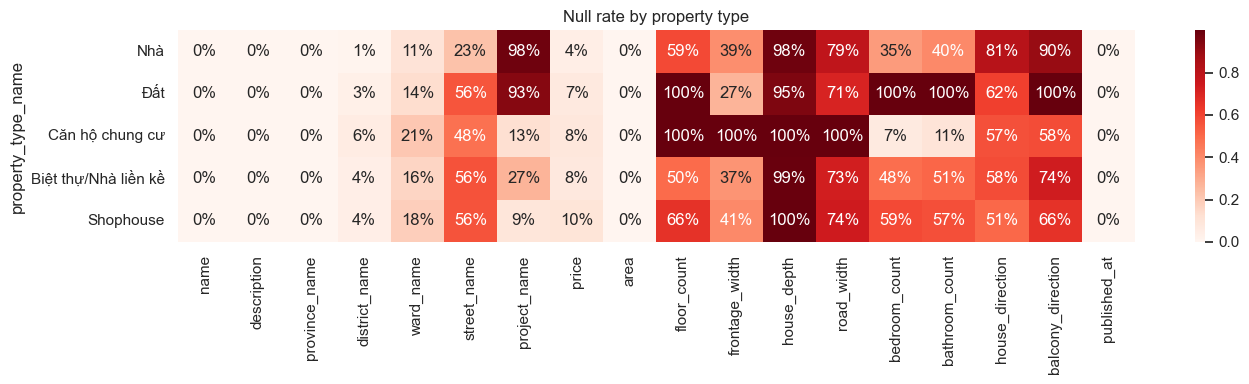
\includegraphics[width=\textwidth]{figures/null_rate_by_property_type.png}
\caption{Null rate of each variable by property type.}
\label{fig:missing-type}
\end{figure}

\paragraph{Validity checks.}
There are 57,320 listings with \texttt{price} equal to zero and none with a negative price. No listing has a non-positive \texttt{area}, and \texttt{floor\_count}, \texttt{bedroom\_count}, and \texttt{bathroom\_count} contain no negative values. Listings without a valid price or area represent 7.88\% of the raw data. This share ranges from 5.2\% (\textit{Nhà}) to 13.6\% (\textit{Shophouse}) across the five property types, and from 4.1\% (Khánh Hòa and Lâm Đồng) to 18.8\% (Hòa Bình) among the 15 provinces with the most listings, so these listings are spread across groups and no single group accounts for most of them.

\paragraph{Temporal, geographic and direction variables.}
The variable \texttt{published\_at} had no missing values, but 22,024 values could not be converted to a timestamp (invalid values were coerced to missing). The parsed values span 1 June 2025 to 30 March 2026. The data contain 63 provinces and 627 districts, and 15 district names appear in more than one province, so \texttt{district\_name} should be used together with \texttt{province\_name}. The direction variables are free text: besides single-direction values, the same direction is sometimes written in two notations (for example, \textit{Đông Nam} and \textit{Đông - Nam}), and a few entries contain several directions, each occurring at most five times. No standardisation was applied at this stage.

\paragraph{Duplicates.}
Listings were flagged as duplicates when they share the normalised \texttt{name}, \texttt{province\_name}, \texttt{district\_name}, \texttt{ward\_name} (lower case, diacritics removed, \textit{đ} mapped to \textit{d}, whitespace collapsed), together with the same \texttt{area} and \texttt{price}, as an earlier listing; the first occurrence is kept. Under this definition, 865,362 listings (24.72\%) are duplicates. The ten most repeated combinations occur between 60 and 121 times each, all in Hồ Chí Minh, and eight of the ten share the same title opening (\textit{xuat canh ban gap}, normalised form).

\paragraph{Extreme prices.}
In the priced, de-duplicated data, the distribution of \texttt{price} on logarithmic axes (Figure~\ref{fig:price-loglog}) is concentrated between about $10^{9}$ and $10^{10}$ VND, with isolated listings below $10^{4}$ VND and above $10^{15}$ VND. The ten lowest prices are between 1,000 and 3,000 VND, and in several of them the title states a different price (for example, a listing recorded at 2,000 VND is titled as 1.6 billion VND). The ten highest range from about $4.49\times10^{14}$ to $2.66\times10^{16}$ VND, and some have very large areas (for example, 999,999~m\textsuperscript{2}). These observations suggest data entry errors, for example in the unit of the price. A range of $[10^{8}, 10^{12}]$ VND (100 million to 1,000 billion VND) was therefore applied; it removes 2,574 listings (0.107\%).

\begin{figure}[H]
\centering
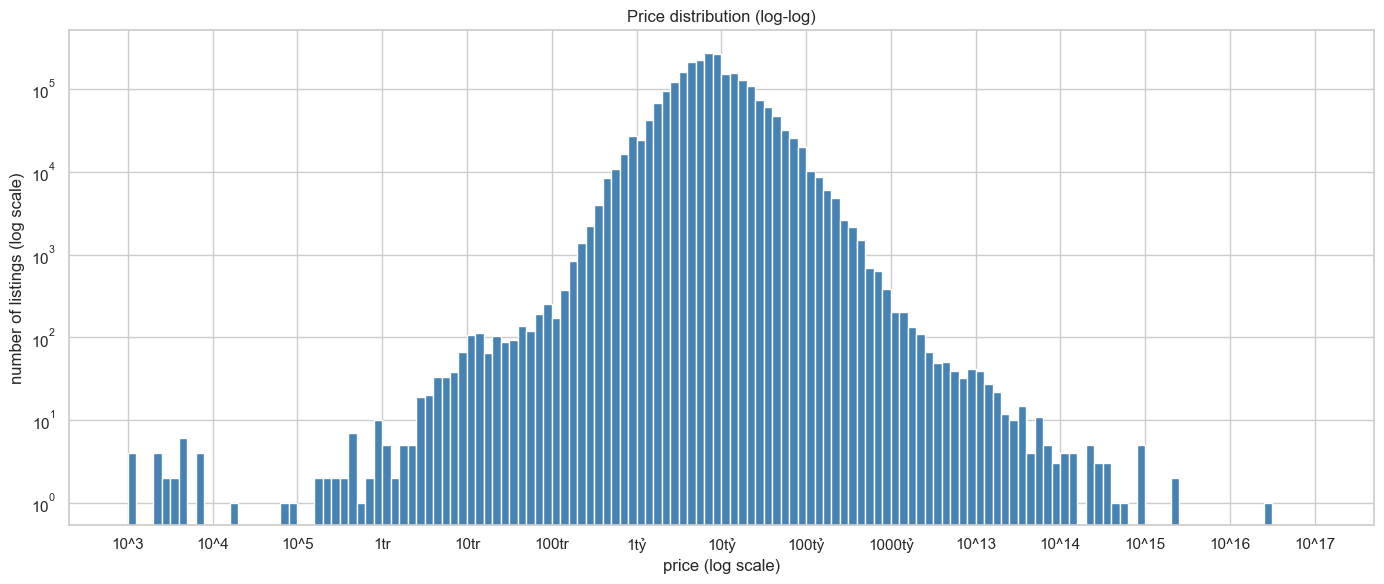
\includegraphics[width=\textwidth]{figures/price_distribution_loglog.png}
\caption{Distribution of asking price after removing invalid prices and duplicates (logarithmic scale on both axes).}
\label{fig:price-loglog}
\end{figure}

\subsection{Analytical Dataset}
\label{subsec:eda-analytical}

The analytical dataset (\texttt{df\_priced}) was built in three steps: retaining listings with $\text{price} > 0$ and $\text{area} > 0$, removing the flagged duplicates, and retaining prices within $[10^{8}, 10^{12}]$ VND. Table~\ref{tab:flow} gives the number of listings after each step. The final dataset contains 2,412,798 listings.

\begin{table}[H]
\centering
\caption{Number of listings after each filtering step.}
\label{tab:flow}
\small
\begin{tabular}{lrr}
\toprule
Step & Listings ($n$) & Removed ($n$) \\
\midrule
Raw data                                     & 3,500,744 & --- \\
Price $> 0$ and area $> 0$                   & 3,224,930 & 275,814 \\
After removing duplicates                    & 2,415,372 & 809,558 \\
Price within $[10^{8}, 10^{12}]$ VND (final) & 2,412,798 &   2,574 \\
\bottomrule
\end{tabular}

\vspace{0.3em}
\footnotesize The number removed in the duplicate step is the difference between the counts before and after the step.
\end{table}

\subsection{Distributions and Relationships in the Analytical Dataset}
\label{subsec:eda-price}

\paragraph{Descriptive profile.}
Table~\ref{tab:describe} reports descriptive statistics of the numeric variables. \texttt{price} and \texttt{area} are available for all listings, whereas the other attributes are available for fewer (from 59,040 for \texttt{house\_depth} to 1,312,102 for \texttt{bedroom\_count}). The median price is 7.4 billion VND and the mean ($1.50\times10^{10}$ VND) is about twice as large, which indicates a right-skewed distribution; \texttt{area} behaves similarly (median 80~m\textsuperscript{2}, mean 416~m\textsuperscript{2}). Several attributes have maxima that are very large relative to their upper quartile, such as \texttt{frontage\_width} ($9.08\times10^{6}$~m), \texttt{road\_width} (18,000~m), \texttt{house\_depth} (15,380~m), \texttt{floor\_count} (255), \texttt{bedroom\_count} (200), and \texttt{bathroom\_count} (168). These values are not plausible for most properties and were not removed or corrected at this stage.

\begin{table}[htbp]
\centering
\caption{Descriptive statistics of numeric variables in the analytical dataset ($N = 2{,}412{,}798$).}
\label{tab:describe}
\scriptsize
\resizebox{\textwidth}{!}{%
\begin{tabular}{lrrrrrrrr}
\toprule
Variable & Count & Mean & Std. dev. & Min & 25\% & 50\% & 75\% & Max \\
\midrule
\texttt{price} (VND)  & 2,412,798 & $1.50\times10^{10}$ & $3.29\times10^{10}$ & $1.00\times10^{8}$ & $4.05\times10^{9}$ & $7.40\times10^{9}$ & $1.43\times10^{10}$ & $1.00\times10^{12}$ \\
\texttt{area} (m\textsuperscript{2}) & 2,412,798 & 416.01 & 92,269.19 & 1.20 & 56.00 & 80.00 & 120.00 & $8.20\times10^{7}$ \\
\texttt{floor\_count} & 517,454 & 3.90 & 1.81 & 1 & 3 & 4 & 5 & 255 \\
\texttt{frontage\_width} (m) & 1,217,495 & 23.38 & 10,391.43 & 0.50 & 4.20 & 5.00 & 7.60 & $9.08\times10^{6}$ \\
\texttt{house\_depth} (m) & 59,040 & 23.84 & 97.32 & 1.00 & 13.40 & 18.75 & 24.75 & 15,380 \\
\texttt{road\_width} (m) & 416,300 & 9.54 & 47.69 & 0.50 & 4.00 & 6.00 & 10.50 & 18,000 \\
\texttt{bedroom\_count} & 1,312,102 & 3.31 & 2.59 & 1 & 2 & 3 & 4 & 200 \\
\texttt{bathroom\_count} & 1,228,546 & 3.06 & 2.55 & 1 & 2 & 2 & 4 & 168 \\
\bottomrule
\end{tabular}}
\end{table}

\paragraph{Distribution of price and area.}
On a base-10 logarithmic scale (Figure~\ref{fig:log-hist}), the distribution of price is unimodal and approximately symmetric, with a mode at about 9.9 (roughly 8 billion VND) and values mainly between 8.5 and 11.5. The distribution of area is unimodal with a mode at about 1.9 to 2.0 (roughly 80 to 100~m\textsuperscript{2}) and a long right tail. Given the right skew shown in Table~\ref{tab:describe}, this supports the use of a log transformation for price.

\begin{figure}[H]
\centering
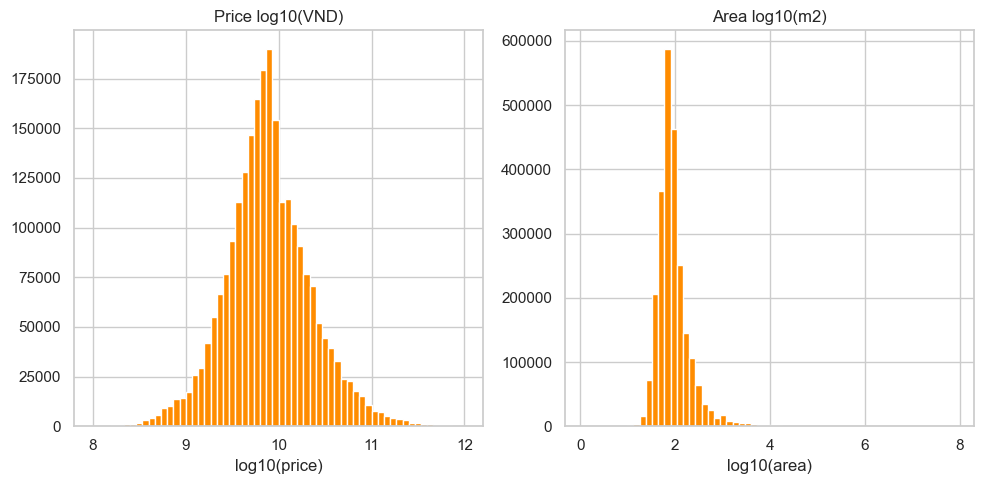
\includegraphics[width=\textwidth]{figures/log10_price_area_hist.png}
\caption{Histograms of $\log_{10}(\text{price})$ (left) and $\log_{10}(\text{area})$ (right).}
\label{fig:log-hist}
\end{figure}

\paragraph{Group coverage.}
Groups with fewer than 100 listings were considered difficult to use as features. All five property types exceed this threshold: houses (1,080,119), land (565,074), apartments (547,956), villas/townhouses (180,047), and shophouses (39,602). Of the 63 provinces, 60 exceed it. Listings are concentrated in Hồ Chí Minh (933,078) and Hà Nội (782,054), which together account for about 71\% of the analytical dataset.

\paragraph{Area and price.}
A scatter plot on logarithmic axes, using a random sample of 20,000 listings (seed 42), is shown in Figure~\ref{fig:scatter}. Most points lie at areas of roughly 30 to 300~m\textsuperscript{2} and prices of roughly $10^{9}$ to $10^{10}$ VND. The cloud shows an upward tendency, so larger areas are generally associated with higher prices, but the dispersion at a given area is wide, and points become sparse above $10^{3}$~m\textsuperscript{2}. This plot is a visual indication only; the strength of the association was not quantified.

\begin{figure}[H]
\centering
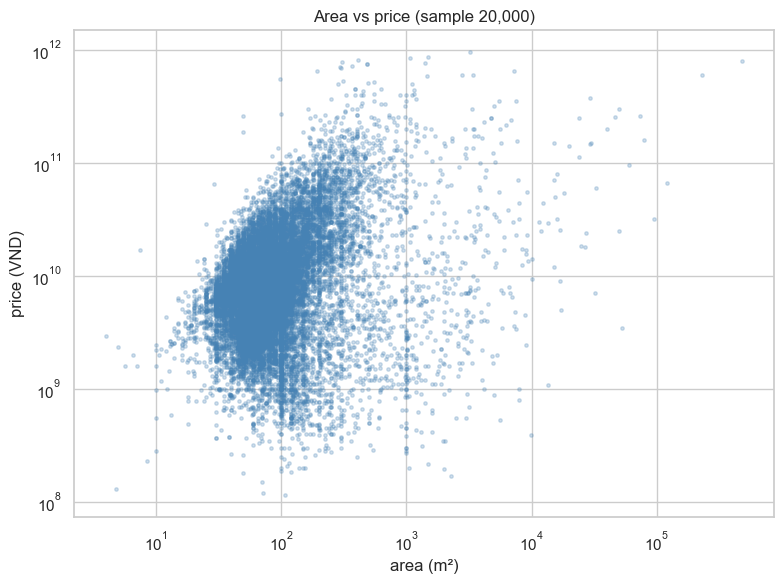
\includegraphics[width=0.75\textwidth]{figures/area_vs_price_scatter.png}
\caption{Area versus asking price on logarithmic axes (random sample of 20,000 listings).}
\label{fig:scatter}
\end{figure}

\paragraph{Price per square metre by property type.}
The price per square metre (\texttt{price\_per\_m2}) is \texttt{price} divided by \texttt{area}. Its $\log_{10}$ distribution for each property type is shown in Figure~\ref{fig:ppm2}, with the horizontal axis restricted to 6--10. Houses and villas/townhouses are centred at higher values (modes at about 8.3 and 8.2, roughly 200 and 160 million VND per m\textsuperscript{2}) than apartments and land (modes at about 7.8). Land has the widest, left-skewed distribution, and apartments the narrowest. Shophouses show two local maxima, at about 7.8--7.9 and 8.2, which may indicate a mix of different kinds of listing (for example, sale and rental); this was not tested and remains a hypothesis.

\begin{figure}[H]
\centering
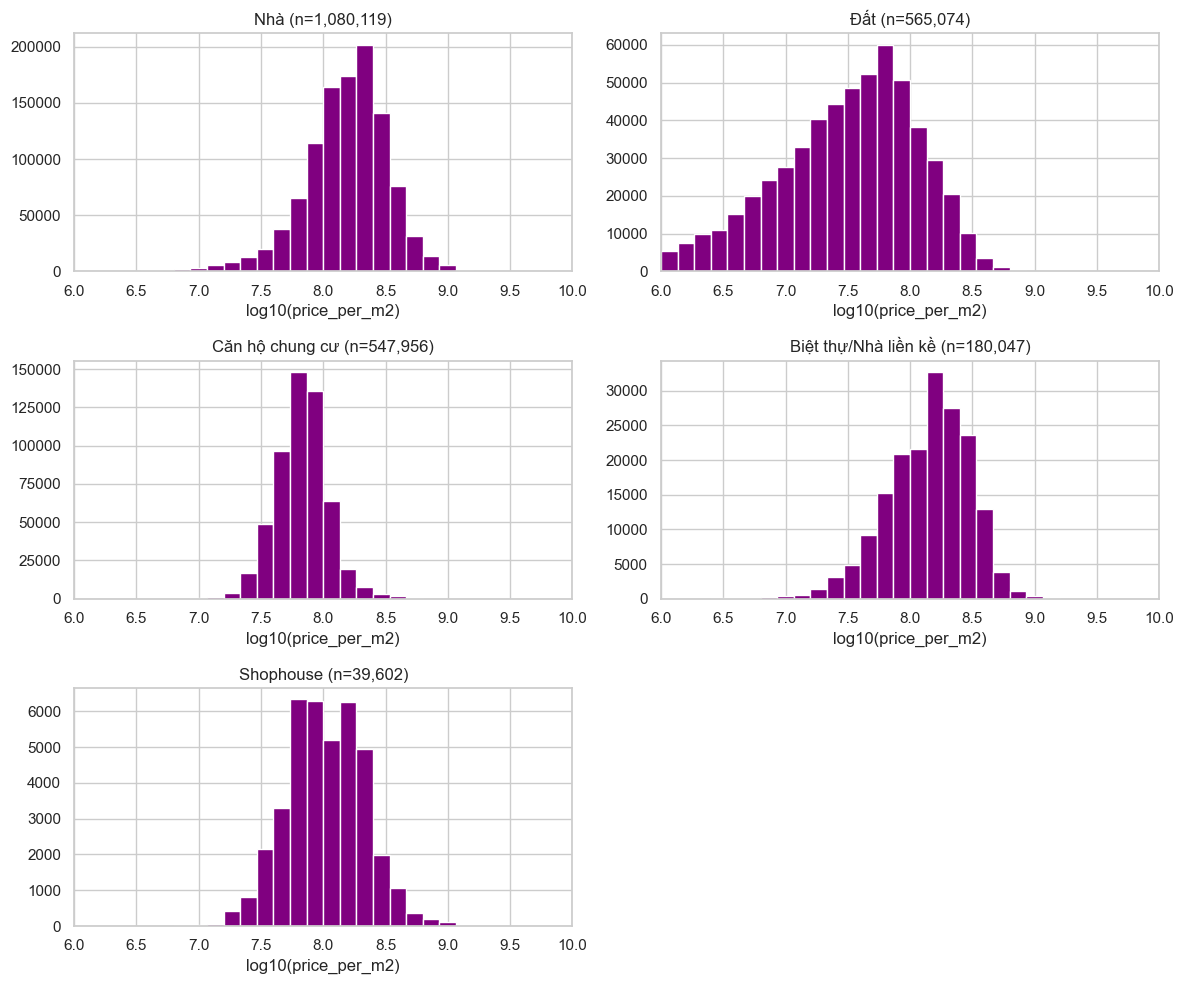
\includegraphics[width=0.9\textwidth]{figures/price_per_m2_by_type.png}
\caption{Distribution of $\log_{10}(\text{price per m}^2)$ by property type (houses $n = 1{,}080{,}119$; land $n = 565{,}074$; apartments $n = 547{,}956$; villas/townhouses $n = 180{,}047$; shophouses $n = 39{,}602$).}
\label{fig:ppm2}
\end{figure}

\subsection{Summary}
\label{subsec:eda-summary}

Missing values are frequent for structural attributes and depend on the property type, 24.72\% of the raw listings were flagged as duplicates, and 7.88\% lack a valid price or area; after filtering, 2,412,798 listings remain. Price and area are right-skewed, and the log transformation of price gives an approximately symmetric distribution, while extreme values in several physical attributes remain untreated. All five property types and 60 of 63 provinces have sufficient listings, although listings are concentrated in two provinces. Area and price show a positive but widely dispersed relationship, and the price per square metre differs by property type.